Differences in gender are central features of economic and social life. This paper investigates how participation in enriched early childhood programs differently enhances the lives of disadvantaged boys and girls, and whether they enhance or reduce life-cycle gender gaps among disadvantaged children.

There is a rich literature in psychology on the greater vulnerability of boys to adverse life conditions. As a group, girls mature earlier, are more resilient to adversity, and perform better in a variety of life tasks.\footnote{See \cite{Schore_2017_IMHJ} for an extensive survey of this literature. Economists have contributed to this literature. See, e.g., \cite{Bertrand_Pan_2013_AEJAE,Autor-etal_2015_Family-Disadvantage}.} Less is known about effective strategies for reducing the vulnerability of boys to disadvantage. 

This paper investigates this question using data from a randomized controlled trial of a prototypical intensive early childhood program that enriched the early lives of disadvantaged children. The program is a template for many current and proposed early interventions.\footnote{Programs inspired by ABC/CARE have been (and are currently being) launched around the world. \citet{Sparling_2010_Highlights} and \citet{Ramey_Ramey_Lanzi_2014_Interventions} list numerous programs based on the ABC/CARE approach. The programs are: IHDP---eight different cities around the U.S. \citep{Spiker-etal_1997_Helping}; Early Head Start and Head Start in the U.S. \citep{Schneider_McDonald-eds_2007_Scale-Up_Vol-1}; John's Hopkins Cerebral Palsy Study in the U.S. \citep{Sparling_2010_Highlights}; Classroom Literacy Interventions and Outcomes (CLIO) study in the U.S. \citep{Sparling_2010_Highlights}; Massachusetts Family Child Care Study \citep{Collins_etal_2010_Massachusetts-Study}; Healthy Child Manitoba Evaluation \citep{Healthy_Child_Manitoba_2015_Starting-Early}; Abecedarian Approach within an Innovative Implementation Framework \citep{Jensen_Nielsen_2016_ABC-Programme-Pilot}; and Building a Bridge into Preschool in Remote Northern Territory Communities in Australia \citep{UMonash_Dataset_2015_URL}. Educare programs are also based on ABC/CARE \citep{Educare_2014_Research_Agenda,Yazejian_Bryant_2012_Educare}.} It starts at 8 weeks of age and continues through age 5. Treatment and control subjects are followed through their mid 30s, with data collected on several dimensions of human development.

There are positive life-cycle impacts of the program for both genders. However, there are substantial differences in impact by gender that vary by domain. The program differentially promotes the labor income, employment, and health of males and reduces their participation in crime. It differentially enhances the cognition, achievement, and educational attainment of girls. We investigate the sources of these differences. Boys placed in childcare benefit relatively more from high-quality center-based care (compared to low-quality center-based care) than girls, although both genders benefit. 

We analyze data from the Carolina Abecedarian Project (ABC) and its closely aligned sister program, the Carolina Approach to Responsive Education (CARE). These programs were conducted in Chapel Hill, North Carolina for a sample of children born between 1972 and 1980. We refer to the combined programs as ABC/CARE.

To preview of our analysis, we report gender differences of outcomes in Figure~\ref{fig:proportion}. We report the proportion of outcomes, by category, for which the males outperform the females (we explain these outcomes in greater detail in the main body of the paper). We do this for the control group and the treatment group separately to establish a baseline gender difference and the value-added of treatment. Control males have higher IQ scores, employment, parental income, and crime than females. They also do better when aggregating across all outcome categories. Treatment drastically narrows the gap between males and females for achievement, with all achievement measures favoring females in the treatment group. Education is another outcome category for which treatment reverses the gender gap. Males have higher educational attainment in the control group with over 50\% of the education outcomes favoring males, although the result is not statistically significant. In the treatment group, however, less than 25\% of the educational outcomes favor males. This pattern also appears for employment outcomes and grouping across all outcome categories. 

\begin{figure}[!htbp]
\centering
\caption{Proportion of Outcomes Males $>$ Females, by Outcome Category}
\label{fig:proportion}
	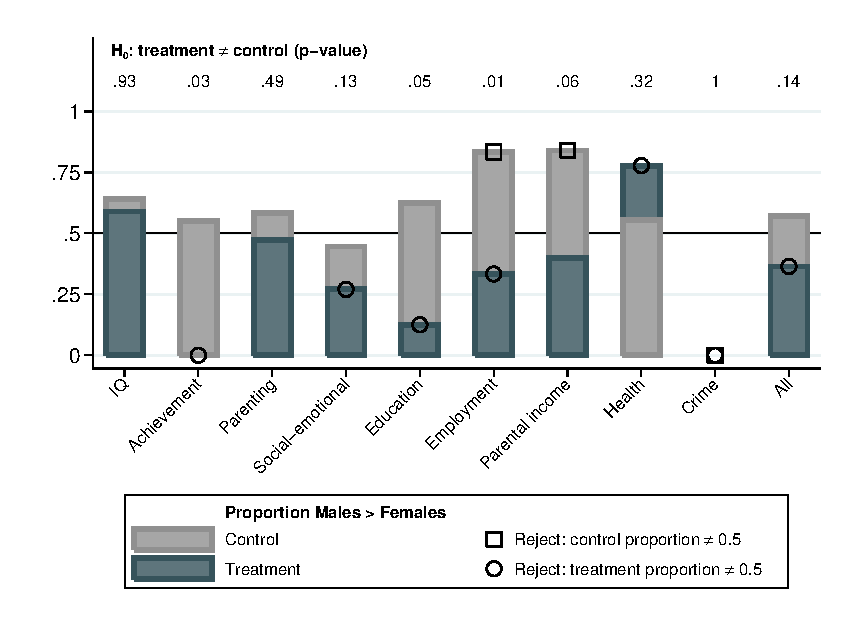
\includegraphics[width=\textwidth]{output/gendergaps-treat-vs-fullcontrol}
\footnotesize \justify
Note: These plots show the proportion of outcomes, by outcome category, for which the males' mean is larger than the females' mean. The standard errors and the $p$-values are computed using 100 bootstraps. The $p$-values are one-sided and test the null hypothesis that the proportion of outcomes is greater than $\frac{1}{2}$. All the variables are coded such that higher values correspond to socially desirable outcomes. The variables for each outcome category are listed in Appendix~\ref{appendix:gdiff-outcome-list}.
\end{figure}

Table~\ref{tab:proportion-table} summarizes the gender gaps in these plots as well as those when considering the alternative setting of the control-group children. In the control group, the proportions of outcomes for which males do better than females is higher than 50\% for most of the categories, although not all are statistically significant. Exceptions include social-emotional skills and crime, in which females surpass males. \textbf{[JJH: Code crime a positive!][This is implemented.]} Treatment reverses the gaps for achievement, education, employment, parental income, and over all outcomes. It widens the gap for health, with treatment leading males to achieve better health outcomes. Considering controls who stay at home, females have slightly better health outcomes. \textbf{[JJH: Why worse health?][Edited]}. Finally, the males who attend lower-quality alternative preschools do not outperform females on any of the outcome categories associated with cognition, education, and parenting. These measurements are concentrated early in life, indicating an early-life disadvantage that enriched early childcare programs partially correct.

\begin{table}[H]
\centering
\caption{Summary of Proportion of Outcomes Males $>$ Females}
\label{tab:proportion-table}
\begin{threeparttable}
\begin{tabular}{l | c |c |c| c}
\toprule
& (1) & (2) & (3) & (4) \\
Category & Control Group  &  Control Group &  Control Group &  Treatment \\
	&				&	Stay at Home		& Alternative Preschool &  Group \\
\midrule  
IQ 								& \checkmark &  \checkmark* & $\times$&\checkmark \\
Achievement						& \checkmark &  \checkmark* &$\times$ & $\times$* \\
Parenting							& \checkmark&  \checkmark* &$\times$ & \checkmark \\
Social-emotional					& $\times$&$=$ &$\times$* &$\times$* \\
Education							& \checkmark&\checkmark & $=$ &$\times$* \\
Employment						&  \checkmark* &  \checkmark* &  \checkmark* &$\times$* \\
Parental income					&  \checkmark* &\checkmark & \checkmark & $\times$\\
Health 							& \checkmark &$\times$ &\checkmark &  \checkmark* \\
Crime							&  \checkmark* &  $=$ & \checkmark* &  \checkmark* \\
\midrule
All								&  \checkmark* &\checkmark*&  $\times$ & $\times$\\
\bottomrule
\end{tabular}
\begin{tablenotes}
\footnotesize
\item Note: This table summarizes comparison of gender gaps across outcome categories by different groups. A \checkmark indicates that the proportion of outcomes in the corresponding category is larger than $\frac{1}{2}$, meaning that males outperform females. A \checkmark* indicates that the proportion is significantly larger than $\frac{1}{2}$. A $\times$ indicates that the proportion is less than $\frac{1}{2}$. A $\times$* indicates that it is significantly less than $\frac{1}{2}$. A $=$ means that the proportion is $\frac{1}{2}$. Column (1) is the difference between males and females in the full control group.  Column (2) is the difference between males and females in the control group only considering those who stayed at home. Column (3) is the difference between males and females in the control group only considering those who attended alternative preschools. Column (4) is the difference between males and females in the treatment group. The variables for each outcome category are listed in Appendix~\ref{appendix:gdiff-outcome-list}.
\end{tablenotes}
\end{threeparttable}
\end{table}

Many studies have shown the potential for early-life interventions to improve the skills of children, especially those from disadvantaged families.\footnote{\citet{Currie_2011_AER,Elango_Hojman_etal_2016_Early-Edu}.} Although several of these studies report effects by gender, the majority do not.\footnote{See \citet{Elango_Hojman_etal_2016_Early-Edu} for a more involved discussion of the literature analyzing early childhood education. Not reporting gender differences is common. Some examples include \citet{Bernal_Keane_2011_JoLE,Cascio_Schanzenbach_2013_ImpactsExpandingAccess,Bitler_et_al_2014_Head_Start_Unpublished,Kline_Walters_2016_QJE}. There are some exceptions: \citet{Heckman_Moon_etal_2010_QE,Campbell_Conti_etal_2014_EarlyChildhoodInvestments,Garcia_Heckman_Leaf_etal_2017_Comp_CBA_Unpublished}.} Pooling males and females can miss potentially large differences in treatment effects. Even if the treatment effects do not significantly differ by gender, early intervention can narrow the gaps present between males and females early in life. 

We summarize (Table~\ref{tab:litreview-table}) work that examines early-life differences between boys and girls. It is generally found that boys are more fragile than girls early in life. While some of these papers consider the family environment, there is a dearth of work studying (1) the effect of low-quality preschool on children\footnote{Although \citet{Kottelenberg-Lehrer_2014_Gender-Effects} study gender gaps, they only consider intact families and do not discuss the quality of the center.} and (2) the interaction of this with family environments. We find that while low-quality programs can deteriorate the parent-child interaction, especially for boys, high-quality programs can enhance it.

\textbf{[We added this table here to highlight it and for quick reference to the added discussion above. We can move this table to the appendix if that is preferred.]}

\begin{sidewaystable}[H]
\centering
\caption{Literature Review on Early Gender Differences}
\label{tab:litreview-table}
\begin{adjustbox}{width=1.05\textwidth}
\begin{threeparttable}
\begin{tabular}{cccccc} \toprule											
\textbf{Paper}	&	\textbf{Program(s)}	&	\textbf{Main Gender-Difference Finding}	&	\textbf{Outcomes}	&	\textbf{Quality of Childcare Setting?} 	&	\textbf{Quality of Home Setting?} 	\\ \midrule
\citet{lundberg2005sons}	&	Literature survey	&	-females: divorce is likely if all children are girls	&	-fertility and divorce	&	No	&	No	\\ 
	&		&	less likely to live with fathers (US), spends more 	&		&		&		\\ 
	&		&	time with mothers	&		&		&		\\ 
	&		&	-males: increase marital stability, increase 	&		&		&		\\ 
	&		&	likelihood of subsequent child	&		&		&		\\ \\ \midrule
\citet{Ou_Reynolds_2010_Mechanisms_CYSR}	&	Chicago Child-Parent Center	&	Differences in treatment effects consequence	&	-educational attainment 	&	No	&	Yes	\\ 
	&	- 1334 youths (682 females, 652 males)	&	of difference in mediators	&	-HS or GED (jointly coded)	&		&		\\ 
	&	- center-based, served 3/4 year olds	&	-male mediators: preschool participation	&		&		&		\\ 
	&	- RCT 	&	-female mediators: family support, abuse/neglect	&		&		&		\\ \\ \midrule
\citet{Bertrand_Pan_2013_AEJAE}	&	ECLS-K (ATUS as complementary)	&	Stark gender differences 	&	-socio-emotional measures	&	No	&	Yes	\\ 
	&	-observational study up to 5th grade	&	- females: better on all socio-emotional measures	&	-grade suspension 	&		&		\\ 
	&		&	(gaps widen when children get older)	&	- tests scores (math and reading)	&		&		\\ 
	&		&	- males: worst at reading but better than math at 	&		&		&		\\ 
	&		&	1st grade	&		&		&		\\ \\ \midrule
\citet{cornwell2013noncognitive}	&	ECLS-K 	&	Gender differences in tests and grades	&	-reading, science, math tests scores 	&	No	&	No	\\ 
	&	-observational study up to 5th grade	&	-males: better in science and math; worst grades	&	-grades	&		&		\\ 
	&		&	overall 	&	-socio-emotional measures	&		&		\\ 
	&		&	females: better reading tests (gap wider than 	&		&		&		\\ 
	&		&	gap with respect to science and math)	&		&		&		\\ 
	&		&	- some but bot all of the gaps disappears when	&		&		&		\\ 
	&		&	accounting for socio-emotional measures 	&		&		&		\\ \\ \midrule
\citet{golsteyn2014gender}	&	Observational study in the Netherlands	&	Gender differences across skills and tests	&	-cognition	&	N/A 	&	No	\\ 
	&	- elementary school children, age 11/12 	&	- males: higher assertiveness and math	&	-socio-emotional measures	&		&		\\ 
	&		&	-females: higher social skills and language	&	-math and language tests	&		&		\\ \\ \midrule
\citet{kottelenberg_Gender}	&	NLSCY	&	-females: better parent-child relationship and 	&	-cognition	&	No	&	Yes	\\ 
	&		&	interactions across diverse measures	&	- socio-emotional outcomes	&		&		\\ 
	&		&	- no precise difference in cognition	&	-parental child relationship and quality of interactions	&		&		\\ 
	&		&		&	-maternal labor supply	&		&		\\ \\ \midrule
\citet{Baker-Milligan_2013_Boy-Girl-Differences}	&	Observational studies in three countries	&	Gender differences in parental investment 	&	-parental investment across different ages	&	No	&	Yes	\\ 
	&	-Canada: NLSCY (ages 1 to 5)	&	-no difference in mother's time at home 	&		&		&		\\ 
	&	-UK: Millennium Cohort Study (ages 1 to 7)	&	-females: more investment in teaching activities	&		&		&		\\ 
	&	-US: ECLS-B (ages 1 to 4)	&	-males: more father's investment at older ages	&		&		&		\\ \\ \midrule
\citet{Magnuson_Kelchen_Duncan_etal_2016_ECRQ}	&	23 programs (meta-analysis)	&	No gender differences, in general	&	-all programs: cognition	&	No	&	No	\\ 
	&	- at least 10 controls	&	- males/females: cognitive benefits	&	-some programs: achievement, behavior,	&		&		\\ 
	&	- from 1960 to 2013	&	- no effect on behavior or mental health	&	adult outcomes	&		&		\\ 
	&	- $<$ 50\%attrition	&		&		&		&		\\ 
	&	- RCTs	&		&		&		&		\\ \\ \midrule
\citet{Schore_2017_IMHJ}	&	Literature survey	&	Sex differences in brain maturation 	&	- brain maturation (right brain development)	&	N/A	&	Yes	\\ 
	&		&	-males: less time spent with mothers, more	&	- daycare behavior	&		&		\\ 
	&		&	sensitive to early infections and endotoxins; 	&	- maternal interaction 	&		&		\\ 
	&		&	respond poorly to daycare settings; amplify stress	&		&		&		\\ 
	&		&	more sensitive to single mother environment	&		&		&		\\ 
	&		&	-females: more rapid brain maturation	&		&		&		\\ \bottomrule
\end{tabular}											
\begin{tablenotes}
\Large
\item Note: This table presents a summary of papers studying early-life gender differences. (1) lists the paper; (2) lists the main program or sample of analysis; (3) lists the main finding with respect to gender differences; (4) the outcomes analyzed; (5) reports if the paper assesses or discusses the quality of the childcare setting; (6) reports if the paper assesses or discusses measures of home quality.
\end{tablenotes}
\end{threeparttable}
\end{adjustbox}
\end{sidewaystable}

This paper reports the treatment effects of ABC/CARE by gender. We report treatment effects comparing treated outcomes with different control conditions, including staying at home or attending other center-based care that was of lower quality than the ABC/CARE program.\footnote{Historical documentation, records, and evidence from knowledgeable individuals indicate that although these alternate centers followed state and federal standards, they were of lower quality than the ABC/CARE program.} Unlike previous studies, we compute treatment effects comparing the treatment group to the control group fixing those in the control group to these two alternate counterfactuals (shown in Table~\ref{tab:proportion-table}).\footnote{Previous studies presenting treatment effects of ABC and CARE include \citet{Ramey_etal_1985_Project-CARE_TiECSE, Clarke_Campbell_1998_ABC_Comparison_ECRQ,Campbell_Pungello_etal_2001_DP,Campbell_Ramey_etal_2002_ADS,Campbell_Wasik_etal_2008_ECRQ,Campbell_Conti_etal_2014_EarlyChildhoodInvestments}.}$^,$\footnote{See \cite{Heckman_1992_randomization}, \cite{Heckman_Hohmann_etal_2000_QJE}, and \cite{Kline_Walters_2016_QJE} for work related to control substitution.} Home care is beneficial for boys. 

This paper unfolds in the following way. In Section~\ref{sec:data}, we describe the experimental data and its special features. We document that a considerable proportion of the control group children attend lower (than treatment) preschools. In Sections~\ref{sec:parameters} and~\ref{sec:combining-functions} we define the estimated treatment effects. Section~\ref{sec:treatment-effects} reports the treatment effects overall and by gender and establishes the existence of sharp gender effects in many categories of outcomes. Section~\ref{sec:gender-differences} discusses differences in the proportions of outcomes favoring men by category. Section~\ref{sec:conclusion} discusses the sources of these differences.

This is one of the features of our paper. It pus together analyzing the effects of early childhood education with gender differences and interprets them jointly. Documenting low-quality preschool alternatives and family environments are important considerations when understanding the effets.

%ee \citet{Beeghly-etal_2017_IMHJ,Dayton_2017_IMHJ,Iruka_2017_IMHJ,Schore_2017_IMHJ} for recent findings on the topic of different development of males and females early in life. 